\documentclass[conference]{IEEEtran}
\usepackage{graphicx}
\usepackage{amsmath}
\usepackage{url}
\usepackage{balance}
\begin{document}
\title{Design and Verification of a Direct-Mapped Cache Controller: Read-Only Prototype and Write-Through Extension}
\author{\IEEEauthorblockN{Naman Jain, Kavya Jain, Lakshay Agrawal, Dhruv Ramani, and Akhilesh Kumar}\\
\IEEEauthorblockA{Modern Computer Architecture, B.Tech (CS\&AI)}}
\maketitle

\begin{abstract}
This paper presents both phases of a synthesizable 1 KB direct-mapped cache. Phase I verified aligned 32-bit reads, tag lookup, and 16-byte refill. Phase II added write-through, write-allocate writes to the same 64-line organization. Self-checking SystemVerilog testbenches verify data, hit/miss status, counters, memory traffic, reset persistence, and write-channel backpressure against an independent reference model. Sequential and repeated read traces achieved 75.00\% and 93.75\% hit rates; 128 uniform random reads achieved 10.16\%. A 128-access mixed trace achieved 83 hits (64.84\%) and 4.06 measured cycles per access. Generic Yosys synthesis found zero design-check problems. These are simulation and generic synthesis results, not FPGA timing claims.
\end{abstract}
\begin{IEEEkeywords}
direct-mapped cache, write-through, write-allocate, SystemVerilog, hit rate, AMAT
\end{IEEEkeywords}

\section{Introduction}
Caches exploit repeated and nearby accesses. Direct mapping gives each block one line, simplifying lookup but allowing repeated conflict replacement \cite{hennessy,patterson}. Phase I measured the read path; Phase II added writes and mixed-access analysis.

\section{Literature Review}
Hennessy and Patterson use hit rate, miss penalty, and average access time to evaluate memory hierarchies \cite{hennessy}; Patterson and Hennessy explain block locality and tag/index/offset mapping \cite{patterson}. Our cache applies these concepts in RTL. Write-through sends every accepted CPU write to memory, simplifying consistency. Write-allocate installs a block after a write miss. Both policies add traffic: every write sends a word, and a write miss also reads a block.

\section{Proposed Solution}
\subsection{Organization and Interfaces}
The data array holds 1,024 bytes in $1024/16=64$ lines, each containing four 32-bit words. A 32-bit byte address uses tag [31:10], index [9:4], and offset [3:0]. The low two bits are zero for supported aligned accesses; bits [3:2] select a word. Each line stores 128 data bits, a 22-bit tag, and one valid bit, for 9,664 storage bits. The CPU presents one request at a time with an address, read/write flag, and optional write data. The cache responds with valid, hit indication, and read data. The simulated memory has separate block-read and word-write handshakes.

\begin{figure}[t]
\centering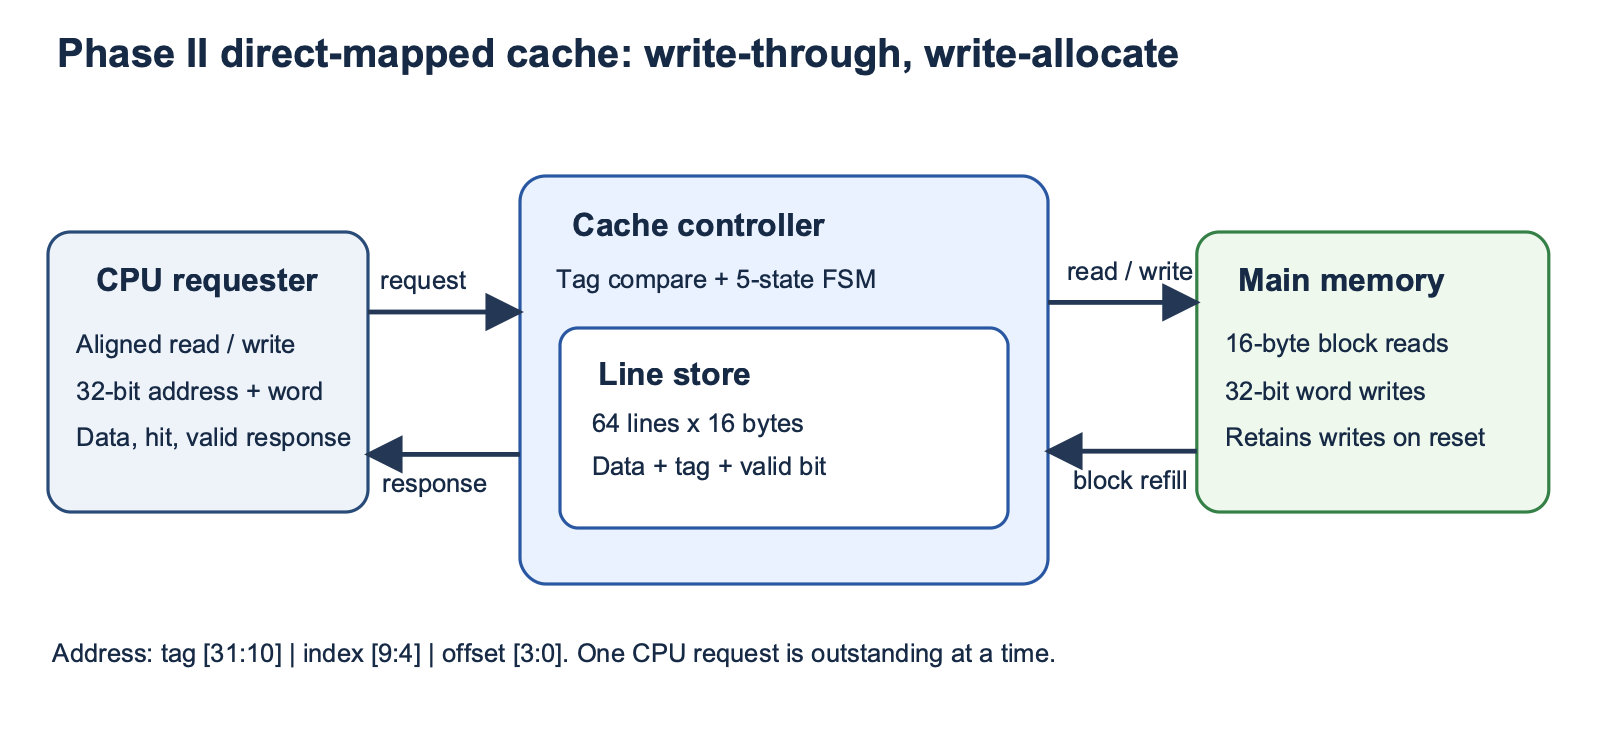
\includegraphics[width=\columnwidth]{../docs/phase2_block_diagram.png}
\caption{Final cache organization. Only the controller and line store are synthesizable; the 4 KB memory is a testbench model.}
\label{fig:p2arch}
\end{figure}

\subsection{Phase I Read-Only Prototype}
The first prototype accepted one aligned read request at a time. On a hit, the selected cached word was returned without a memory request. On a miss, the controller requested an aligned 16-byte block, refilled the indexed line, and returned the selected word. Its implemented states were \texttt{IDLE}, \texttt{LOOKUP}, \texttt{MISS\_REQUEST}, and \texttt{MISS\_WAIT}. Reset cleared valid bits and hit/miss counters; data and tag arrays did not need reset because invalid lines could not hit.

\subsection{Phase II Read and Write Policy}
The final controller preserves the read behavior. On a write hit, it waits until the word-write channel accepts the word; on that same edge it updates the cached word and then responds. On a write miss, it first fetches the old block, replaces the addressed word in the refill data, writes the block/tag/valid fields, then sends the 32-bit word to memory and responds only after acceptance. A write response carries zero read data. Cache reset invalidates lines and clears counters; it does not erase the test memory's written words.

\subsection{Final Controller and Storage}
The Phase II controller has five implemented states: \texttt{IDLE}, \texttt{LOOKUP}, \texttt{MISS\_REQUEST}, \texttt{MISS\_WAIT}, and \texttt{WRITE\_REQUEST}. In \texttt{IDLE} it captures one request. \texttt{LOOKUP} compares valid and tag, increments one of the hit/miss counters, and chooses the read response, refill, or write path. \texttt{MISS\_REQUEST} holds the aligned block address until accepted. \texttt{MISS\_WAIT} refills on the returned block. \texttt{WRITE\_REQUEST} holds address/data/valid stable under backpressure and completes the CPU write after the memory handshake. The line store has an entire-block refill port and a selected-word update port; refill has priority if both are asserted.

\section{Verification Method}
The 4 KB memory model initializes word $i$ to $\mathrm{A5000000}+i$ and returns blocks after a three-cycle delay. Phase I tested cold misses, block hits, sequential and repeated reads, and conflicts between 0x00000000 and 0x00000400. Phase II added a seeded 128-address uniform random-read trace and word writes retained across cache reset. Its testbench compares every response with independent Python reference vectors and checks counters, one block read per miss, one word write per CPU write, and exclusive memory requests. Directed cases cover write hits/misses, eviction, adjacent-word preservation, and post-reset readback. A separate 128-operation mixed trace tests locality and conflicts. A stalled write tests stable address/data and delayed CPU response. Any mismatch calls \texttt{\$fatal}.

\section{Results and Discussion}
Table~\ref{tab:p1results} reports Phase I read traces. Hits take 2 measured cycles and misses 7 under the included memory model. The miss ratio is $M/(H+M)=1-H/(H+M)$; it is 25.00\% for sequential, 6.25\% for repeated, and 100.00\% for alternating conflicts. The latter always misses in the same cache, averaging 7.00 cycles versus 3.25 and 2.31 cycles for sequential and repeated reads.

\begin{table}[t]
\caption{Phase I Read-Only Simulation Results}
\label{tab:p1results}
\centering\footnotesize
\begin{tabular}{lrrrr}
\hline
Trace & Reads & H/M & Hit rate & Cycles/op\\\hline
Directed & 7 & 4/3 & 57.14\% & 4.14\\
Sequential & 16 & 12/4 & 75.00\% & 3.25\\
Repeated & 16 & 15/1 & 93.75\% & 2.31\\
Conflict & 16 & 0/16 & 0.00\% & 7.00\\\hline
\end{tabular}
\end{table}

Table~\ref{tab:p2results} reports Phase II traces. Uniform random reads have 13 hits and 115 misses: 10.16\% hit ratio, 89.84\% miss ratio, and $[13(2)+115(7)]/128=6.49$ measured cycles per access. The mixed trace has 89 reads and 39 writes: 68 read hits, 21 read misses, 15 write hits, and 24 write misses. Its miss ratio is 35.16\%, and traffic is $45\times16+39\times4=876$ bytes. Block fills can fetch unused words.

\begin{table}[t]
\caption{Phase II Simulation Results}
\label{tab:p2results}
\centering\footnotesize
\begin{tabular}{lrrrr}
\hline
Trace & Ops & H/M & Hit rate & Cycles/op\\\hline
Directed mixed & 9 & 5/4 & 55.56\% & 4.44\\
Random reads & 128 & 13/115 & 10.16\% & 6.49\\
Seeded mixed & 128 & 83/45 & 64.84\% & 4.06\\\hline
\end{tabular}
\end{table}

For the included memory model and handshake, read hit, read miss, write hit, and write miss take 2, 7, 3, and 8 measured request-to-response cycles, respectively, without added backpressure. The mixed-trace average memory access time (AMAT) measured in these cycles is
\begin{equation}
\mathrm{AMAT}=\frac{68(2)+21(7)+15(3)+24(8)}{128}=4.0625.
\end{equation}
This trace-specific average includes controller handshakes. Directed readback verified persistence after cache reset and conflict eviction; stalled writes produced no early response.

\subsection{Synthesis and Limits}
Yosys 0.71+post synthesized the cache RTL with hierarchy flattening and reported zero design-check problems for both phases. The read-only Phase I design reported 29,525 generic cells, and the Phase II read/write design 55,448; each count includes one scope-information pseudo cell. The increase reflects added write selection and control in this flow, not a device-area comparison. No FPGA target, technology library, or clock constraint was supplied. FPGA LUT/BRAM usage and maximum operating frequency remain unmeasured.

\balance
\section{Individual Contributions}
Assigned review areas are: M1 Naman Jain, controller/integration; M2 Kavya Jain, line storage/address mapping; M3 Lakshay Agrawal, memory/write protocol; M4 Dhruv Ramani, verification; and M5 Akhilesh Kumar, reference model/results/report. The local build does not establish personal authorship. Each member must confirm actual work and make their own meaningful repository commits before submission.

\section{Conclusion}
Phase I verified read lookup, refill, and conflicts. Phase II added write-through, write-allocate support and passed directed, reset-persistence, backpressure, and 128-operation mixed-trace checks. The mixed trace measured 64.84\% hits and 4.06 cycles per access. FPGA timing/resource analysis still requires a target device and tool flow. The preserved logs and waveforms support the viva demonstration.

\begin{thebibliography}{3}
\bibitem{hennessy} J. L. Hennessy and D. A. Patterson, \emph{Computer Architecture: A Quantitative Approach}, 6th ed. Morgan Kaufmann, 2017.
\bibitem{patterson} D. A. Patterson and J. L. Hennessy, \emph{Computer Organization and Design RISC-V Edition: The Hardware Software Interface}, 2nd ed. Morgan Kaufmann, 2020.
\bibitem{yosys} YosysHQ, ``Yosys synthesis commands,'' Yosys documentation. [Online]. Available: \url{https://yosyshq.readthedocs.io/projects/yosys/en/latest/using_yosys/synthesis/synth.html}
\end{thebibliography}
\end{document}
